\documentclass[a4paper,twocolumn]{article} % Document type

\ifx\pdfoutput\undefined
    %Use old Latex if PDFLatex does not work
   \usepackage[dvips]{graphicx}% To get graphics working
   \DeclareGraphicsExtensions{.eps} % Encapsulated PostScript
 \else
    %Use PDFLatex
   \usepackage[pdftex]{graphicx}% To get graphics working
   \DeclareGraphicsExtensions{.pdf,.jpg,.png,.mps} % Portable Document Format, Joint Photographic Experts Group, Portable Network Graphics, MetaPost
   \pdfcompresslevel=9
\fi
\usepackage{subcaption}
\usepackage{amsmath,amssymb}   % Contains mathematical symbols
\usepackage[ansinew]{inputenc} % Input encoding, identical to Windows 1252
\usepackage[english]{babel}    % Language
%\usepackage[round,authoryear]{natbib}  %Nice author (year) citations
\usepackage[square,numbers]{natbib}     %Nice numbered citations
%\bibliographystyle{unsrtnat}           %Unsorted bibliography
\bibliographystyle{plainnat}            %Sorted bibliography

\addtolength{\topmargin}{-30mm}% Removes 30mm from the top margin
\addtolength{\textheight}{30mm}% Adds it to the text height


\begin{document}               % Begins the document

\title{Reproducing Sequential Attention for Feature Selection}
\author{Gary Wang, Hank Lai \\ N16132087, N16132079 \\ n16132087@gs.ncku.edu.tw, n16132079@gs.ncku.edu.tw} 
%\date{2010-10-10}             % If you want to set the date yourself.

\maketitle                     % Generates the title




%%%%%%%%%%%%%%%%%%%%%%%%%%%%%%%%%%%%%%%%%%%%%%%%%%%%%%%%%%%%%%%%%%%%%%%%%%%%%%%%%%%
% Instructions regarding the report
%%%%%%%%%%%%%%%%%%%%%%%%%%%%%%%%%%%%%%%%%%%%%%%%%%%%%%%%%%%%%%%%%%%%%%%%%%%%%%%%%%%

\section{Introduction}

Feature selection is essential for improving interpretability, generalization, and efficiency in high-dimensional learning tasks.
 However, As noted in a review by Nordling (2013, Chapter 5.2) have noted, it remains a challenging problem due to 
computational limits and sensitivity to noise. Classical methods such as LASSO and greedy search either fail to capture feature interactions or lack robustness.

Sequential Attention (SA) proposes a novel attention-based relaxation of greedy selection that models conditional importance adaptively. 
In this study, we aim to reproduce SA and evaluate whether it consistently outperforms classical methods 
like Sequential LASSO and Group LASSO.


\section{Problem Description}

Given a dataset $X \in \mathbb{R}^{n \times d}$ and labels $y \in \mathbb{R}^n$, the goal of feature selection is to find a subset $S \subseteq \{1, ..., d\}$ of $k$ features that maximize the predictive performance of a model $f(X_S)$.

Classical methods often ignore the marginal gain of features conditioned on already-selected features.
 SA addresses this by learning attention scores in a sequential manner. We evaluate whether SA more effectively 
identifies relevant subsets by comparing its classification accuracy and stability to that of Sequential LASSO and Group LASSO on benchmark datasets.

\section{Methods}
\subsection{Sequential Attention Algorithm}
% Description of algorithm, possibly Algorithm 1 from paper



\subsection{Experimental Setup}
% Dataset info, network architecture, optimizer, seeds, etc.

\section{Results}
\subsection{Dataset Overview}

\begin{figure*}[h!]
    \centering

    % === SA
    \begin{subfigure}[t]{0.23\linewidth}
        
\includegraphics[width=\linewidth]{figures/reference_features_sa.png}
        \caption*{SA Reference}
    \end{subfigure}
    \hfill
    \begin{subfigure}[t]{0.23\linewidth}
        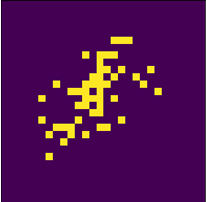
\includegraphics[width=\linewidth]{figures/reference_features_gl.png}
        \caption*{GL Reference}
    \end{subfigure}
    \hfill
    \begin{subfigure}[t]{0.23\linewidth}
        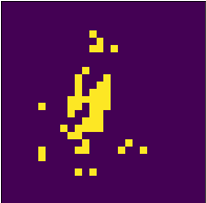
\includegraphics[width=\linewidth]{figures/reference_features_omp.png}
        \caption*{OMP Reference}
    \end{subfigure}
    \hfill
    \begin{subfigure}[t]{0.23\linewidth}
        
\includegraphics[width=\linewidth]{figures/reference_features_seql.png}
        \caption*{SEQL Reference}
    \end{subfigure}

    \vspace{1em}

    \begin{subfigure}[t]{0.23\linewidth}
        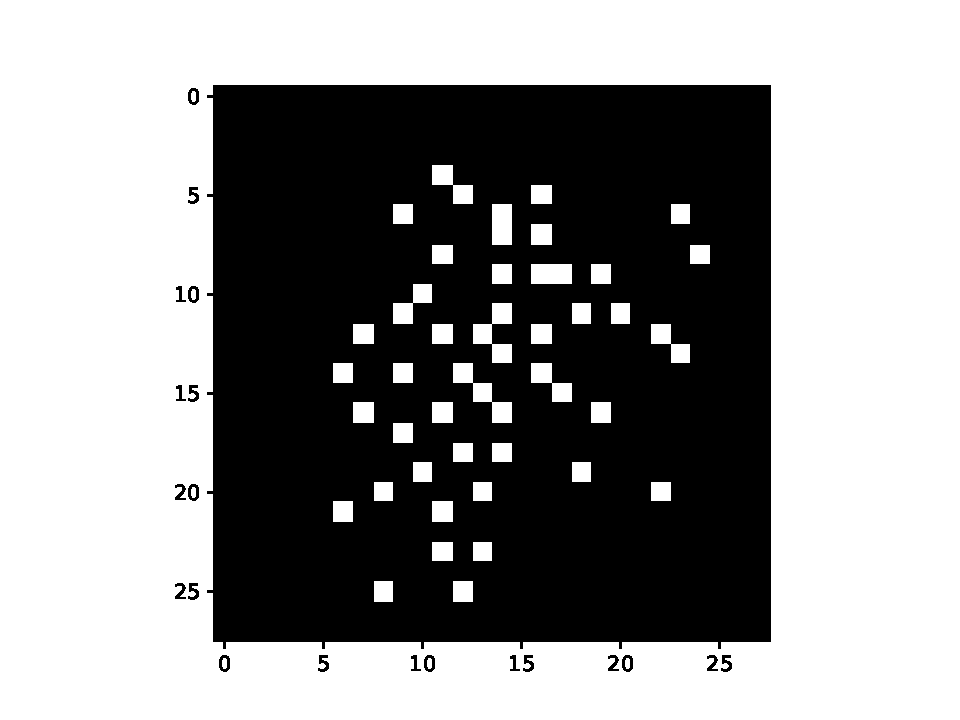
\includegraphics[width=\linewidth]{figures/best_seed_sa.pdf}
        \caption*{SA Best}
    \end{subfigure}
    \hfill
    \begin{subfigure}[t]{0.23\linewidth}
        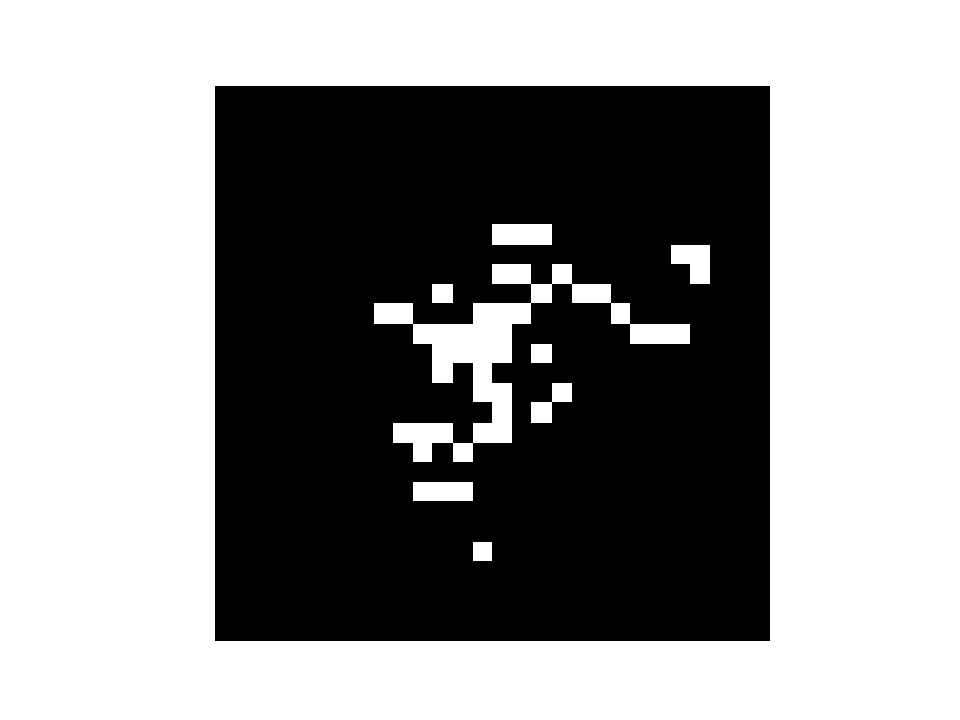
\includegraphics[width=\linewidth]{figures/best_seed_gl.pdf}
        \caption*{GL Best}
    \end{subfigure}
    \hfill
    \begin{subfigure}[t]{0.23\linewidth}
        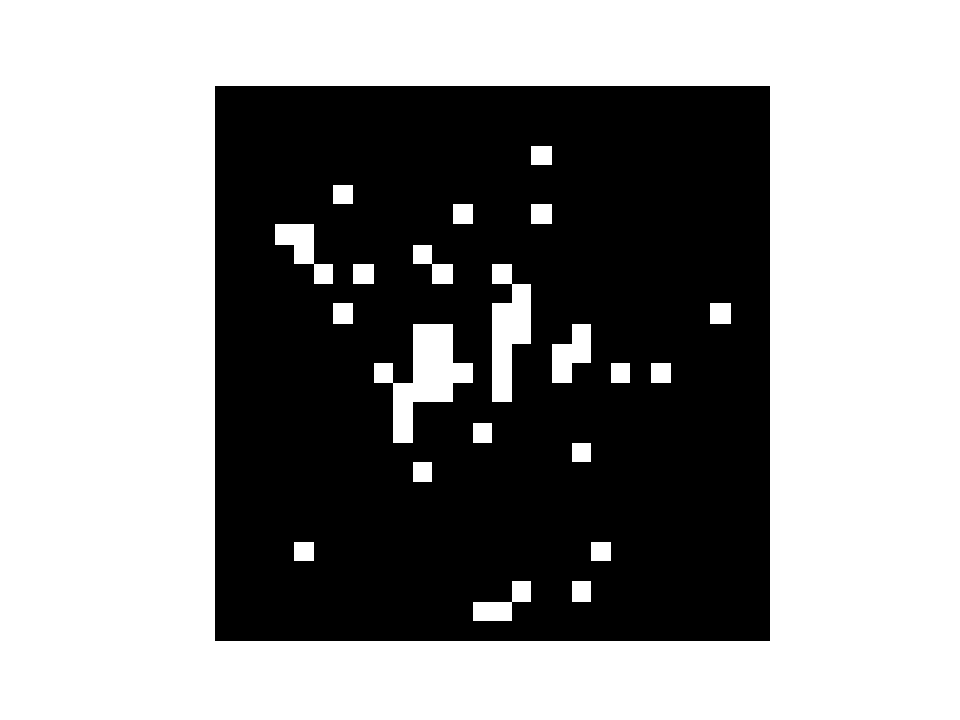
\includegraphics[width=\linewidth]{figures/best_seed_omp.pdf}
        \caption*{OMP Best}
    \end{subfigure}
    \hfill
    \begin{subfigure}[t]{0.23\linewidth}
        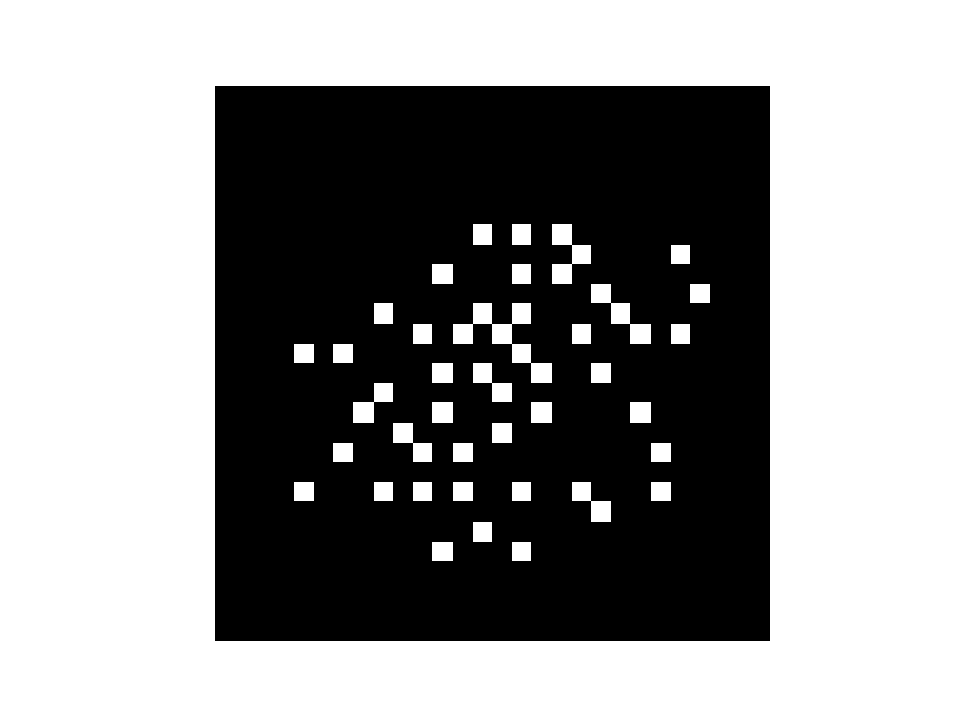
\includegraphics[width=\linewidth]{figures/best_seed_seql.pdf}
        \caption*{SEQL Best}
    \end{subfigure}

    \caption{Top row: reference masks; bottom row: best-seed selection results for each method.}
    \label{fig:feature_masks}
\end{figure*}

\begin{table}[ht]
    \centering
    \begin{tabular}{lcc}
        \hline
        \textbf{Method} & \textbf{Best Seed} & \textbf{SSIM} \\
        \hline
        SA    & 3 & 0.0992 \\
        GL    & 5 & 0.3249 \\
        OMP   & 1 & 0.1401 \\
        SEQL  & 2 & 0.0874 \\
        \hline
    \end{tabular}
    \caption{SSIM values for the best seed selected by each method.}
    \label{tab:ssim_results}
\end{table}

\begin{table*}[ht]
\centering
\resizebox{\textwidth}{!}{
\begin{tabular}{lc|cc|cc}
\hline
\textbf{Dataset} & \textbf{Our results} & \textbf{Lemhadri (2021)~\cite{lemhadri2021lassonet}} & \textbf{p-value} & \textbf{Yasuda (2023)} & \textbf{p-value} \\
\hline
Mice Protein     & 0.989 $ \pm $ 0.008 & 0.990 & 0.7623 & 0.963 & 0.0017 \\
MNIST            & 0.973 $ \pm $ 0.001 & 0.928 & 0.0000 & 0.953 & 0.0000 \\
MNIST-Fashion    & 0.874 $ \pm $ 0.003 & 0.833 & 0.0000 & 0.869 & 0.0297 \\
ISOLET           & 0.950 $ \pm $ 0.003 & 0.953 & 0.1269 & 0.961 & 0.0015 \\
COIL-20          & 0.994 $ \pm $ 0.002 & 0.996 & 0.1381 & 0.986 & 0.0005 \\
Activity         & 0.942 $ \pm $ 0.002 & 0.853 & 0.0000 & 0.954 & 0.0002 \\
\hline
\end{tabular}
}
\caption{Comparison of accuracy using all features. p-values are from one-sample t-tests against Lemhadri et al. and Yasuda et al.'s reported means.}
\label{tab:all-feature-pval}
\end{table*}

\begin{table*}[ht]
\centering
\resizebox{\textwidth}{!}{%
\begin{tabular}{lcccccc}
\hline
\textbf{Dataset} & \textbf{SA} & \textbf{LLY} & \textbf{GL} & \textbf{SL} & \textbf{OMP} & \textbf{CAE} \\
\hline
Mice Protein    & 0.993 $\pm$ 0.008 & 0.981 $\pm$ 0.005 & 0.985 $\pm$ 0.005 & 0.984 $\pm$ 0.008 & 0.994 $\pm$ 0.008 & 0.956 $\pm$ 0.012 \\
MNIST           & 0.956 $\pm$ 0.002 & 0.944 $\pm$ 0.001 & 0.937 $\pm$ 0.003 & 0.959 $\pm$ 0.001 & 0.912 $\pm$ 0.004 & 0.909 $\pm$ 0.007 \\
MNIST-Fashion   & 0.854 $\pm$ 0.003 & 0.843 $\pm$ 0.005 & 0.834 $\pm$ 0.004 & 0.854 $\pm$ 0.003 & 0.829 $\pm$ 0.008 & 0.839 $\pm$ 0.003 \\
ISOLET          & 0.920 $\pm$ 0.006 & 0.866 $\pm$ 0.012 & 0.906 $\pm$ 0.006 & 0.920 $\pm$ 0.003 & 0.727 $\pm$ 0.026 & 0.893 $\pm$ 0.011 \\
COIL-20         & 0.997 $\pm$ 0.001 & 0.994 $\pm$ 0.002 & 0.997 $\pm$ 0.004 & 0.988 $\pm$ 0.005 & 0.967 $\pm$ 0.014 & 0.972 $\pm$ 0.007 \\
Activity        & 0.931 $\pm$ 0.004 & 0.897 $\pm$ 0.025 & 0.933 $\pm$ 0.002 & 0.931 $\pm$ 0.003 & 0.905 $\pm$ 0.013 & 0.921 $\pm$ 0.001 \\
\hline
\end{tabular}
}
\caption{Feature selection accuracy (mean $\pm$ std) on small-scale datasets}
\label{tab:feature-selection}
\end{table*}

\begin{table*}[ht]
\centering
\resizebox{\textwidth}{!}{%
\begin{tabular}{lcccccccccc}
\hline
\textbf{Dataset} & \textbf{SA} & \textbf{p-value} & \textbf{LLY} & \textbf{p-value} & \textbf{GL} & \textbf{p-value} & \textbf{SL} & \textbf{p-value} & \textbf{OMP} & \textbf{p-value} \\
\hline
Mice Protein   & 0.994 $\pm$ 0.005 & 0.8915 & 0.982 $\pm$ 0.009 & 0.7567 & -              & -      & -              & -      & 0.994 $\pm$ 0.005 & 0.8998 \\
MNIST          & 0.890 $\pm$ 0.016 & 0.0007 & 0.848 $\pm$ 0.026 & 0.0012 & 0.973 $\pm$ 0.001 & 0.0000 & 0.914 $\pm$ 0.005 & 0.0000 & 0.890 $\pm$ 0.016 & 0.0355 \\
MNIST-Fashion  & 0.764 $\pm$ 0.029 & 0.0022 & 0.809 $\pm$ 0.011 & 0.0011 & 0.877 $\pm$ 0.005 & 0.0000 & 0.802 $\pm$ 0.008 & 0.0000 & 0.764 $\pm$ 0.029 & 0.0068 \\
ISOLET         & 0.850 $\pm$ 0.018 & 0.0007 & 0.843 $\pm$ 0.017 & 0.0377 & -              & -      & -              & -      & 0.850 $\pm$ 0.018 & 0.0000 \\
COIL-20        & 0.983 $\pm$ 0.008 & 0.0167 & 0.987 $\pm$ 0.005 & 0.0210 & 0.997 $\pm$ 0.003 & 0.9056 & -              & -      & 0.983 $\pm$ 0.008 & 0.0369 \\
Activity       & 0.864 $\pm$ 0.034 & 0.0117 & 0.869 $\pm$ 0.053 & 0.3099 & -              & -      & -              & -      & 0.864 $\pm$ 0.034 & 0.0542 \\
\hline
\end{tabular}
}
\caption{Comparison of mean accuracy and p-values between methods and paper baselines across datasets. Method order follows original paper: SA, LLY, GL, SL, OMP.}
\label{tab:method-comparison}
\end{table*}


\subsection{Feature Selection Accuracy}
% Accuracy table or plots for k=50 features


\subsection{Statistical Validation}
% t-test or p-value results table if needed
\subsection{VISUALIZATION OF SELECTED MNIST FEATURES}
To select the seed whose selected feature distribution most closely resembles that shown in the original Figure 5, we computed both Intersection over Union (IoU) and Structural Similarity Index (SSIM) between our visualizations and those reported in the paper. IoU quantifies the overlap in selected features, while SSIM captures the perceptual similarity in structural patterns. Using both metrics allows us to evaluate the alignment from both a positional and visual perspective, and choose the seed with the most consistent spatial feature selection.


\section{Discussion}
% Analysis of differences, strengths, weaknesses, generalization, possible error sources
\subsection{ Small-scale experiments}

\subsection{ Large-scale experiments}
We encountered difficulties reproducing the large-scale experiment presented in Figure 4 of the original paper. Specifically, the Criteo Click dataset used in that experiment requires approximately 1TB of disk space. 
Due to hardware limitations on both our local machines and available servers, we were unable to process and store the full dataset. 
As a result, we were not able to reproduce the large-scale results associated with this figure.

\section{Conclusion}
% Summary of what was reproduced and whether claims hold

\bibliographystyle{ieeetr}
\bibliography{references}


% Optionally include appendix
\clearpage
\appendix
\section*{Appendix}
\section{Hyperparameters}
% Learning rate, batch size, etc.

\section{Additional Figures}
% Supplementary plots

\end{document}      % End of the document
